\documentclass{exam}
\usepackage[utf8]{inputenc}
\usepackage{lmodern}
\usepackage{microtype}

% \usepackage[parfill]{parskip}
\usepackage[dvipsnames]{xcolor}
\usepackage{amsmath}
\usepackage{amsfonts}
\usepackage{amsthm}
\usepackage{siunitx}
\DeclareSIUnit\year{yr}
\DeclareSIUnit\foot{ft}
\DeclareSIUnit\litre{\liter}

\usepackage{skull}

\usepackage{pgfplots}
\usepgfplotslibrary{polar}
\pgfplotsset{compat=1.11}
\usepgfplotslibrary{statistics}
\usepackage{graphicx}
\usepackage{sidecap}
\sidecaptionvpos{figure}{c}
\usepackage{float}
\usepackage{gensymb}
\usepackage{tkz-euclide}
\usetkzobj{all}
\usepackage{commath}
\usepackage{hyperref}
\usepackage{enumitem}
\usepackage{wasysym}
\usepackage{multicol}
\usepackage{mathtools}
\usepackage{tcolorbox}
\usepackage{tabularx}
\usepackage[version=4]{mhchem}
\usepackage{changepage}
\usepackage{listings}
\lstset{basicstyle=\ttfamily\linespread{0.8}\small}

\renewcommand*{\thefootnote}{\fnsymbol{footnote}}

\newtheorem*{thm}{Theorem}
\newtheorem*{iden}{Identity}
\newtheorem*{lemma}{Lemma}
\newtheorem{obs}{Observation}
\theoremstyle{definition}
\newtheorem*{defn}{Definition}
\newtheorem*{ex}{Example}
\newtheorem{con}{Construction}
\newtheorem*{alg}{Algorithm}

\newtheoremstyle{break}
  {\topsep}{\topsep}%
  {\itshape}{}%
  {\bfseries}{}%
  {\newline}{}%
\theoremstyle{break}
\newtheorem*{bthm}{Theorem}

% russian integral
\usepackage{scalerel}
\DeclareMathOperator*{\rint}{\scalerel*{\rotatebox{17}{$\!\int\!$}}{\int}}

% \DeclareMathOperator*{\rint}{\int}

\pgfplotsset{vasymptote/.style={
    before end axis/.append code={
        \draw[densely dashed] ({rel axis cs:0,0} -| {axis cs:#1,0})
        -- ({rel axis cs:0,1} -| {axis cs:#1,0});
    }
}}

% \pointsinrightmargin
\boxedpoints
\pointname{}

\newcommand{\questioA}{\question[\texttt{\textbf{\color{Cerulean} A}}]}
\newcommand{\questioM}{\question[\texttt{\textbf{\color{PineGreen} M}}]}
\newcommand{\questioE}{\question[\texttt{\textbf{\color{WildStrawberry} E}}]}
\newcommand{\questioS}{\question[\texttt{\textbf{\color{Goldenrod} S}}]}
\newcommand{\questioO}{\question[\texttt{\textbf{\color{BurntOrange} O}}]}

\newcommand{\parA}{\part[\texttt{\textbf{\color{Cerulean} A}}]}
\newcommand{\parM}{\part[\texttt{\textbf{\color{PineGreen} M}}]}
\newcommand{\parE}{\part[\texttt{\textbf{\color{WildStrawberry} E}}]}
\newcommand{\parS}{\part[\texttt{\textbf{\color{Goldenrod} S}}]}
\newcommand{\parO}{\part[\texttt{\textbf{\color{BurntOrange} O}}]}

\newcommand{\subparA}{\subpart[\texttt{\textbf{\color{Cerulean} A}}]}
\newcommand{\subparM}{\subpart[\texttt{\textbf{\color{PineGreen} M}}]}
\newcommand{\subparE}{\subpart[\texttt{\textbf{\color{WildStrawberry} E}}]}
\newcommand{\subparS}{\subpart[\texttt{\textbf{\color{Goldenrod} S}}]}
\newcommand{\subparO}{\subpart[\texttt{\textbf{\color{BurntOrange} O}}]}

\newcommand{\mainHeader}[2]{\section*{NCEA Level 2 Mathematics\\#1. #2}}
\newcommand{\mainHeaderHw}[2]{\section*{NCEA Level 2 Mathematics (Homework)\\#1. #2}}
\newcommand{\seealso}[1]{\begin{center}\emph{See also #1.}\end{center}}
\newcommand{\drills}[1]{\begin{center}\emph{Drill problems: #1.}\end{center}}
\newcommand{\basedon}[1]{\begin{center}\emph{Notes largely based on #1.}\end{center}}


\begin{document}

\mainHeader{14}{Anti-differentiation}
The final mathematical topic that we will look at with regard to calculus is the inverse operation to
differentiation: given a slope function (a derivative), we will find the original function.

\begin{ex}
  Suppose that we know that the derivative of some function is the function $ f' $ given by $ f'(x) = 3x^2 + 2x + 1 $. By reversing the power
  rule for derivatives, we can see that if we take $ f_0 $ to be $ f_0(x) = x^3 + x^2 + x $ then we get the desired derivative (i.e. $ f_0' = f' $).
  On the other hand, any function $ f_C $ such that $ f_C(x) = x^3 + x^2 + x + C $ also has the same derivative.
\end{ex}

From this example, we make two main observations:
\begin{obs}
  If we know a differentiation rule, like $ ax^r \mapsto arx^{r - 1} $, then we can reverse it and say that if the derivative
  looks like $ ax^r $ then the original function looks like $ \frac{a}{r + 1}x^{r + 1} $.
\end{obs}

\begin{obs}
  Given any derivative $ f' $, we have infinitely many functions that have $ f' $ as their derivative: if
  one is $ f $, then $ f + C $ for any constant $ C $ also has $ f' $ as its derivative, because
  \begin{displaymath}
    (f + C)' = f' + C' = f' + 0 = f'.
  \end{displaymath}
\end{obs}

The set of antiderivatives of some function $ f' $ is denoted by
\begin{displaymath}
  \rint f'(x) \dif{x} = f(x) + C.
\end{displaymath}
The notation is unfortunate, but the best way to view it this year is as a pair of brackets: $ \rint $ and $ \dif{x} $. The
mathematical operation of taking an antiderivative is called indefinite integration --- if taking a function and finding its
slope is splitting the function up into infinitely many pieces, then taking the antiderivative is packing all those infinitely
many pieces back together into one integrated whole.

\begin{ex}
  Suppose that it is known that the function $ f $
  \begin{itemize}
    \item has a derivative $ f'(x) = 3x^5 + 4x^3 + 2x + 1 $, and
    \item has a graph which passes through the point $ (2,1) $.
  \end{itemize}
  Then we know that all the possible candidates for $ f $ are given by
  \begin{displaymath}
    \rint 3x^5 + 4x^3 + 2x + 1 \dif{x} = \frac{3}{6}x^6 + \frac{4}{4}x^4 + \frac{2}{2}x^2 + \frac{1}{1}x^1 + C = \frac{x^6}{2} + x^4 + x^2 + x + C.
  \end{displaymath}
  We also know that $ f(2) = 1 $, so:
  \begin{gather*}
    1 = \frac{2^6}{2} + 2^4 + 2^2 + 2 + C \\
    1 = 2^5 + 2^4 + 2^2 + 2 + C = 32 + 16 + 4 + 2 + C = 54 + C\\
    C = 1 - 54 = -53
  \end{gather*}
  and hence $ f(x) = \frac{x^6}{2} + x^4 + x^2 + x - 53 $.
\end{ex}

There is not much more to say about integration at this stage, because at Level 2 the geometric meaning of integration is no
longer examinable. Suffice it to say, the operation of integration (as you will learn next year) is far deeper and more interesting
than it first appears. The final problems in this week's problem set are an indication of this.

\subsection*{Questions}
\begin{questions}
  \question Find three functions that have derivatives equal to $ x^2 - x $.
  \question Find an antiderivative of $ f(x) = 25x^4 + 12x^3 - x^{-2} $.
  \question Evaluate $ \rint 12z^3 + 18z^{-4} \dif{z} $.
  \question Show that $ x^3 + 3x + C $ is an antiderivative of $ 3x^2 + 3 $.
  \question Show that
            \begin{equation}
              \rint 470x^4 + 2x + 1 + 6x^{-3} \dif{x} = 94x^5 + x^2 + x - 3x^{-2} + C.
            \end{equation}
  \question Evaluate the following indefinite integral:
             \begin{displaymath}
               \rint -x^6 - \frac{1}{3\sqrt{x}} + \frac{x^{19}}{47} - \frac{2}{x^{-\frac{4}{5}}} \dif{x}
             \end{displaymath}
  \question Given the slope functions below, draw the antiderivative of each which passes through $ (0,0) $.
    \begin{parts}
      \part \fbox{\begin{tikzpicture}
              \begin{axis}[
                axis lines = center,
                xlabel = $ x $,
                ylabel = {$ y = f'(x) $},
                xmin = -3, xmax = 5,
                ymin = -8, ymax = 40
              ]
                \addplot[domain = -3:5, color = blue, samples = 100] {x^2 + 3*x - 3};
              \end{axis}
            \end{tikzpicture}}
            \fbox{\begin{tikzpicture}
              \begin{axis}[
                axis lines = center,
                xmin = -3, xmax = 5,
                ymin = -24, ymax = 24
              ]
%                 \addplot[domain = -3:5, color = blue, samples = 100] {x^2 + 3*x - 3};
              \end{axis}
            \end{tikzpicture}}
      \part \fbox{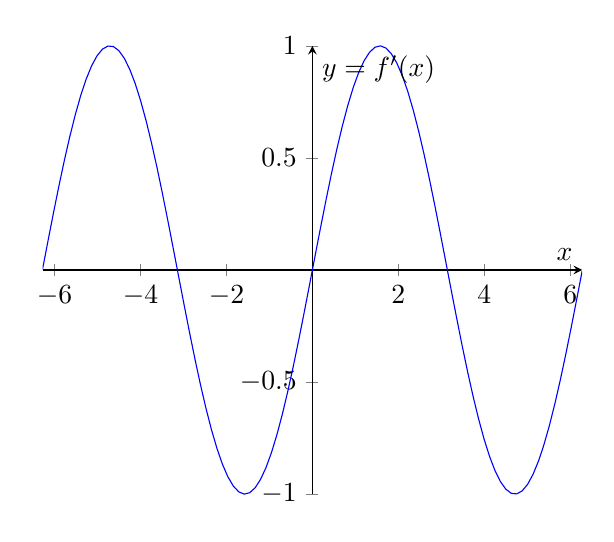
\begin{tikzpicture}
              \begin{axis}[
                axis lines = center,
                xlabel = $ x $,
                ylabel = {$ y = f'(x) $},
                xmin = -6.28, xmax = 6.28,
                ymin = -1, ymax = 1
              ]
                \addplot[domain = -6.28:6.28, color = blue, samples = 100] {sin(deg(x))};
              \end{axis}
            \end{tikzpicture}}
            \fbox{\begin{tikzpicture}
              \begin{axis}[
                axis lines = center,
                xmin = -6.28, xmax = 6.28,
                ymin = -1, ymax = 1
              ]
%                 \addplot[domain = -6.28:6.28, color = blue, samples = 100] {sin(deg(x))};
              \end{axis}
            \end{tikzpicture}}
      \part \fbox{\begin{tikzpicture}
              \begin{axis}[
                axis lines = center,
                xlabel = $ x $,
                ylabel = {$ y = f'(x) $},
                xmin = -1, xmax = 5,
                ymin = -15, ymax = 30
              ]
                \addplot[domain = -1:5, color = blue] {-(x - 1)*(x - 2)*(x - 4)};
              \end{axis}
            \end{tikzpicture}}
            \fbox{\begin{tikzpicture}
              \begin{axis}[
                axis lines = center,
                xmin = -1, xmax = 5,
                ymin = -22, ymax = 23
              ]
%                 \addplot[domain = -1:5, color = blue] {-(x - 1)*(x - 2)*(x - 4)};
              \end{axis}
            \end{tikzpicture}}
      \part \fbox{\begin{tikzpicture}
              \begin{axis}[
                axis lines = center,
                xlabel = $ x $,
                ylabel = {$ y = f'(x) $},
                xmin = -1, xmax = 5,
                ymin = -5, ymax = 5
              ]
                \addplot[domain = -1:2, color = blue] {2*x - 3};
                \addplot[domain = 2:5, color = blue] {0.5*(x-2)^2 + 1};
              \end{axis}
            \end{tikzpicture}}
            \fbox{\begin{tikzpicture}
              \begin{axis}[
                axis lines = center,
                xmin = -1, xmax = 5,
                ymin = -5, ymax = 5
              ]
%                 \addplot[domain = -1:2, color = blue] {2*x - 3};
%                 \addplot[domain = 2:5, color = blue] {0.5*(x-2)^2 + 1};
              \end{axis}
            \end{tikzpicture}}
    \end{parts}
  \question
    \begin{parts}
      \part By drawing graphs, show that it is plausible that $ \od{}{x} \cos x = -\sin x $. (You may assume for the remainder of this question
            that this derivative is correct.)
      \part Find all possible functions $ \psi $ such that
            \begin{displaymath}
              \psi'(x) = 4 \sin x + \frac{2x^5 - \sqrt{x}}{x}.
            \end{displaymath}
      \part Suppose that we know that $ \psi(0) = -8 $. Find $ \psi $.
    \end{parts}
  \question Find $ g $ if $ g'(x) = x \sqrt{x} $ and $ g(1) =  2 $.
  \question Suppose that $ \theta $ is a function of $ x $ such that
            \begin{displaymath}
              \theta'(x) = 8x^3 + 3x^2 + ax,
            \end{displaymath}
            where $ a $ is a constant. Given that $ \theta(0) = 9 $ and $ \theta(-1) = 14 $, find $ \theta $ and $ a $.
  \question Find $ f(x) $ if $ f''(x) = -2 + 12x - 12x^2 $, $ f(0) = 4 $, and $ f'(0) = 12 $.
  \question Suppose that $ f $ is a function of $ x $ given by $ f(x) = x^3 - Ax^2 + 3x - B $, where $ A $ and $ B $ are real constants,
            which passes through $ (0,-4) $ and has a critical point at $ x = 1 $. Find $ f(x) $ exactly.
  \question Suppose that $ y $ is a function of $ x $ given by
            \begin{displaymath}
              y = x^3 + Bx^2 + Cx + 1,
            \end{displaymath}
            and that the graph of $ y $ has a minimum at $ (3,0) $.

            Find $ B $ and $ C $.
  \question Every function which is made up of bits of the form $ ax^r $ added up can be differentiated using the power rule.
            However, the same is not true for differentiation.
    \begin{parts}
      \part Show that no such function $ f $ differentiates to give $ f'(x) = \frac{1}{x} $. (Hint: try to integrate using the
            reverse power rule).
      \part It is a consequence of a theorem of analysis that a function $ f $ exists so that $ f'(x) = \frac{1}{x} $, even though
            it is not of the form above. Given the following graph of $ f' $, draw the graph of $ y = f(x) $ if $ f(1) = 0 $.
            \fbox{\begin{tikzpicture}
              \begin{axis}[
                axis lines = center,
                xlabel = $ x $,
                ylabel = {$ y = f'(x) $},
                xmin = 0, xmax = 5,
                ymin = -1, ymax = 10
              ]
                \addplot[domain = 0.01:5, color = blue, samples = 100] {1/x};
              \end{axis}
            \end{tikzpicture}}
            \fbox{\begin{tikzpicture}
              \begin{axis}[
                axis lines = center,
                xmin = 0, xmax = 5,
                ymin = -5, ymax = 6
              ]
%                 \addplot[domain = -3:5, color = blue, samples = 100] {x^2 + 3*x - 3};
              \end{axis}
            \end{tikzpicture}}
      \part The function which you graphed in part (b) is given the special name $ \ln $; so you have drawn the graph of $ y = \ln(x) $.
            Let us consider the inverse function of $ \ln $, which we will call $ \mathrm{nl} $ for the time being (because it's like ln
            backwards). Given the rule that $ \od{y}{x} = \frac{1}{\od{x}{y}} $, we can find the derivative of $ \mathrm{nl} $ from the
            derivative of $ \ln $.
        \begin{subparts}
          \subpart Write $ x = \ln y $, and give $ \od{x}{y} $.
          \subpart Hence show that $ \od{y}{x} = x $.
          \subpart Conclude that, since $ x = \ln y \iff y = \mathrm{nl}\thinspace x $, it must be the case
                   that $ \od{}{x} \mathrm{nl}\thinspace x = \mathrm{nl}\thinspace x $.
        \end{subparts}
      \part So $ \mathrm{nl} $ is its own derivative --- a situation we already looked at! Clearly $ \mathrm{nl} $ is not the zero function; we
            saw that there was only one other function which was its own derivative. What was it? (Hint: check the end of sheet 11.)
      \part If $ \ln $ is the inverse of the type of function that you found $ \mathrm{nl} $ to be, what kind of function is it?
      \part The letters $ \ln $ stand for \emph{logarithme naturel} (French). Why do you think this is?
    \end{parts}
  \question (Advertisement for Level 3!)
    \begin{parts}
      \part Draw the line $ y = 2t + 1 $ and use geometry to find the area under
            this line, above the $ t$-axis, and between the vertical lines $ t = 1 $
            and $ t = 3 $.
      \part If $ x > 1 $, let $ A(x) $ be the area of the region that lies under the line $ y = 2t + 1 $
            between $ t = 1 $ and $ t = x $. Sketch this region and use geometry to find an expression
            for $ A(x) $.
      \part Find $ A'(x) $. What do you notice?
    \end{parts}
\end{questions}

\end{document}
